\chapter{Successful case studies}


FALTA DESARROLLAR LOS DOS ÚLTIMOS PUNTOS



\section{CMS at the LHC}

High-energy physicists working at the Compact Muon Solenoid (CMS) detector at the LHC, that generates more than 100 datacentres in a three-tier model and generates around 10PB of data each year, are benefiting from a NoSQL database management system that gives them unified access to data from a huge variety of sources (from relational and non-relational data sources, such as relational databases, document-oriented databases, blogs, wikis, file systems and customised applications). The team providing data management to the CMS Cern project has built a system using MongoDB in preference to relational database technologies and other non-relational options. The reasons to select MongoDB were:

\begin{itemize}
\item Dynamic queries support
\item full indexes
\item auto-sharding
\end{itemize}

Several years ago the data management group at the CMS confronted a data discovery problem, with a variety of databases necessitating a user interface that would hide the complexity of the underlying architecture from the physicists. There was a vast variety of distributed databases and different formats (HTML, XML, JSON files, etc.).

%
\paragraph{Data Aggregation System}
To provide the ability to search and aggregate information across this complex data landscape CMS's Data Management and Workflow Management (DMWM) project created a data aggregation system (DAS), built on MongoDB. 

Valentin Kuznetsov, a research associate at Cornell University, says that ``there was nothing specific to the system related to our experiment'', so it can be deduced that this MongoDB approach is extensible. 

%%%%%

\section{PanDA Workload Management System}


\begin{figure}
\centering
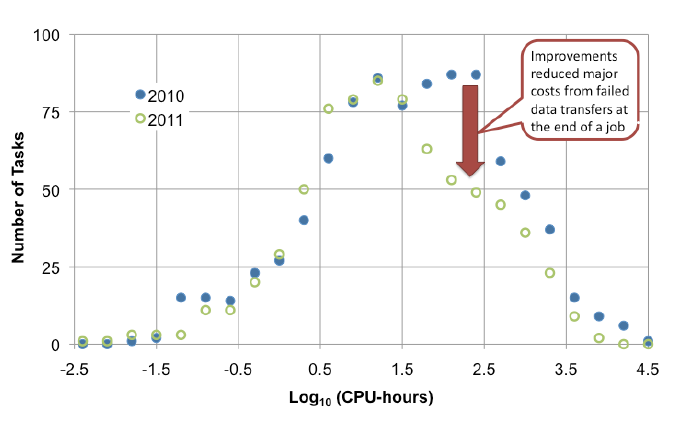
\includegraphics[width=14cm,height=8cm]{images/panda.png}
\caption{Weibull distribution of CPU-hours used to recover job failures in petascale data processing, from \href{https://sharepoint.anl.gov/hep/HEP\%20Accomplishments/Highlights_101212.pdf}{Argonne National Library}}
\end{figure}






%%%%%%%%%%%%%%%%%%%%


\section{Measuring radiation levels in Seattle}



Researchers at the University of Washington utilized the Cloudant NoSQL database as part of an experiment that determined radiation levels in Seattle as a result of the recent Fukushima nuclear disaster are “well below alarming limits.” The research team, which includes Cloudant Founder and Chief Scientist Mike Miller (his other title is research associate professor of physics), studied particles captured from the five air filters at the university’s Physics and Astronomy building and used Cloudant’s CouchDB-based BigCouch database to store and process the data from its experiments.

